\chapter{Background} \label{c:Background}
My goal is the same as in the paper \textit{\acrshort{snh}}, namely to animate human-like characters. More precisely, the focus is on the behaviour of the character's flesh. This chapter serves as an introduction into the mathematical as well as physical background, needed to understand the upcoming calculations and conclusions. At the beginning of this chapter, I will define the notation and convention used throughout this whole thesis. Next, I will give insights in the mathematics used and present some of the concepts used in continuum mechanics. However, I will not include each proof explicitly, as there are already many good resources for an interested reader.

\section{Notation and Convention}
At first, I will declare the notation used in this thesis to avoid misunderstandings. I will use the common notation used in continuum mechanics taken from the book \textit{Continuum Mechanics} \cite{Spencer1980}. Additionally, I will include some more specific declarations formulated and used by the authors of the paper \textit{\acrshort{snh}}.


\subsection{General Notation}
Scalars are represented by regular, normal-weight variables such as $a$, whereas tensors and matrices are represented by upper-case bold letters such as for example $\textbf{A}$. Vectors will be denoted by bold lower-case variables like $\textbf{a}$. 


\subsection{Tensor Notation}
Furthermore, I will use the tensor notation used in \textit{\acrshort{snh}}. They decided to define the vectorization vec(\cdot) as column-wise flattening of a matrix into a vector (\cite{Smith:2018:SNF:3191713.3180491}, 12:5) similar to Golub and Van Loan (2012) (\cite{golub2012matrix}).

In order to indicate that I am dealing with a vectorized matrix, I will use the symbol $\check{\cdot}$ as shown in the following equation:

\[
\mathbf{A} = \begin{bmatrix} a & c \\ b & d \end{bmatrix} \qquad \operatorname{vec}(\mathbf{A}) = \mathbf{\check{a}} = \begin{bmatrix} a \\ b \\ c \\ d \end{bmatrix}
\]

Additionally, I will have to deal with $4^{th}$ order tensors in a form of matrix-of-matrices. These matrices are denoted by using blackboard bold:

\[
\mathbb{A} = 
\left[\begin{array}{cc}{\begin{bmatrix} a & c \\ b & d \end{bmatrix}} & {\begin{bmatrix} i & k \\ j & l \end{bmatrix}} \\ {\begin{bmatrix} e & g \\ f & h \end{bmatrix}} & {\begin{bmatrix} m & o \\ n & p \end{bmatrix}}\end{array}\right]
=
\left[\begin{array}{cc}{\left[\mathbf{A}_{00}\right]} & {\left[\mathbf{A}_{01}\right]} \\ {\left[\mathbf{A}_{10}\right]} & {\left[\mathbf{A}_{11}\right]}\end{array}\right]
\]

We can now vectorize $\mathbb{A}$ and get the following result:

\[
\operatorname{vec}(\mathbb{A}) = \left[ \,\operatorname{vec}\left(\mathbf{A}_{00}\right)\, \bigg| \,\operatorname{vec}\left(\mathbf{A}_{10}\right)\, \bigg| \,\operatorname{vec}\left(\mathbf{A}_{01}\right)\, \bigg| \,\operatorname{vec}\left(\mathbf{A}_{11}\right)\, \right] = \mathbf{\check{A}}
\]

This term above is equivalent to

\[
\mathbf{\check{A}}=\left[\begin{array}{llll}{a} & {e} & {i} & {m} \\ {b} & {f} & {j} & {n} \\ {c} & {g} & {k} & {o} \\ {d} & {h} & {l} & {p}\end{array}\right].
\]

The advantage of this form is that we can write several expressions as a cross product. I will need this property later to simplify complicated expressions and calculations.


\subsection{Summary}
Here is a quick overview of the introduced notation:
\begin{align*}
\text{a}&: \text{Scalar} \\
\mathbf{A}&: \text{Matrix or tensor} \\
\mathbf{a}&: \text{Vector} \\
\mathbf{\check{a}}&: \text{Vectorized matrix (also written as vec($\mathbb{A}$))} \\
\mathbf{\check{A}}&: \text{matrix-of-matrices}
\end{align*}


\section{Mathematical Background}
Since mathematics play an important role in the field of interest, the first step is to build a solid background before diving further into more complex calculations. This section covers all the important concepts used later in the calculations. A basic understanding of linear algebra is assumed.

\subsection{Singular Value Decomposition}

The \acrlong{svd} (\acrshort{svd}) will play an important role in the formulation of the deformation gradient. It represents the best possible approximation of a given matrix by a matrix of low rank. This approximation can be looked at as a compression of the data given (\cite{LiesenMehrmann2015}, p. 295). Firstly we need to define what singular values are.

\begin{definition}[\textbf{Singular Values}]
\label{singular_values}
The singular values of a matrix $\mathbf{A}$ $\in$ $\mathbb{R}^{m x n}$ are the square roots of the eigenvalues of $\mathbf{AA}^{\intercal}$.
\end{definition}

The theorem of the singular value decomposition tells us that we can factor every m-by-n matrix into one orthogonal m-by-m, one diagonal m-by-n and one orthogonal n-by-n matrix. More formally:

\begin{theorem}[\textbf{The \acrshort{svd} Theorem}]
\label{SVD}
Let $\mathbf{A}$ $\in$ $\mathbb{R}^{m x n}$ be a matrix having r positive singular values, m $\geq$ n. Then there exist orthogonal matrices $\mathbf{U}$ $\in$ $\mathbb{R}^{m x m}$, $\mathbf{V}$ $\in$ $\mathbb{R}^{n x n}$ and a diagonal matrix $\mathbf{\tilde{\Sigma}}$ $\in$ $\mathbb{R}^{m x n}$ such that
\begin{align*}
\mathbf{A} &= \mathbf{U \tilde{\Sigma} V^\intercal} \\
\mathbf{\tilde{\Sigma}} &= \left[ \begin{array}{cc} \mathbf{\Sigma} & 0 \\ 0 & 0 \end{array} \right]
\end{align*}
where $\mathbf{\Sigma}$ = diag ($\sigma_1$, $\sigma_2$, . . . , $\sigma_r$), and $\sigma_1$ $\geq$ $\sigma_2$ $\geq$ · · · $\geq$ $\sigma_r$ $>$ 0 are the positive singular values of $\mathbf{A}$.
\end{theorem}

This definition and theorem were taken from \textit{Numerical linear algebra with applications: Using MATLAB} (\cite{ford2014numerical}, p.113, p.300).


\subsection{Polar Decomposition}
Another theorem we will use in the next sections is the Polar Decomposition Theorem.

\begin{theorem}[\textbf{The Polar Decomposition Theorem}]
\label{PD}

Let $\mathbf{F}$ be a non-singular square matrix. Then $\mathbf{F}$ can be decomposed uniquely into either of the following two products
\[
\mathbf{F} = \mathbf{RU}, \quad \mathbf{F} = \mathbf{VR}
\]
where $\mathbf{R}$ is orthogonal and $\mathbf{U}$ and $\mathbf{V}$ are positive definite symmetric matrices.
\end{theorem}

This theorem was taken from \textit{Continuum Mechanics} in which they include the proof for $3 \times 3$ matrices (\cite{Spencer1980}, p.12).

\subsection{Frobenius Norm}

\begin{definition}[\textbf{Frobenius Norm}]
\label{FN}
Let \textbf{A} be a (m $\times$ n) matrix in the real or complex domain. Then the Frobenius norm is defined as 
\[
\| \mathbf{A} \|_{F} := \sqrt{\sum\limits_{i=1}^{m} \sum\limits_{j=1}^{n} |a_{ij}|^2}.
\]
\end{definition}

We can further represent the norm with the trace of the matrix, in which $\mathbf{A}^*$ is the conjugate transpose of \textbf{A}. Going from there, we can use the \acrshort{svd} of \textbf{A} and write the norm with respect to the singular values of \textbf{A}, denoted by $\sigma_i$:
\begin{equation} \label{eq:FN}
\| \mathbf{A} \|_{F} = \sqrt{\operatorname{trace}(\mathbf{A} \mathbf{A}^*)} = \sqrt{\sum\limits_{i=1}^{\operatorname{min}\{m,n\}} \sigma_i^2}
\end{equation}


\section{Continuum Mechanics}
In this section, I will give a broad introduction into the field of Continuum Mechanics. In Continuum Mechanics, we are less interested in small particles like atoms or molecules of an object but rather in pieces of matter which are in comparison very large. The reason for this is that the calculation for the behaviour of individual atoms is very difficult for larger systems. We are therefore concerned with the mechanical behavior of solids and fluids on the macroscopic scale and we treat material as uniformly distribeted throughout regions of space. With this approach, it is possible to define quantities such as displacement, density, etc. as continuous functions of position (\cite{Spencer1980}, p. 1).


\subsection{Deformation}
In continuum mechanics the term \textit{strain} is used as a measure of deformation and we denote \textit{stress} as the force per unit area. If we apply a force over an object, the object itself undergoes a deformation. This behavior is intuitively clear. Graphically, we can imagine a deformation with the help of a two dimensional deformation map as shown in Fig. \ref{fig:deformationmap}. The ellipse on the left side represents an object in its rest state. A function $\phi$ maps this rest state of the ellipse to a deformed state as shown on the right side.

\begin{figure}[!htbp]
	\centering
	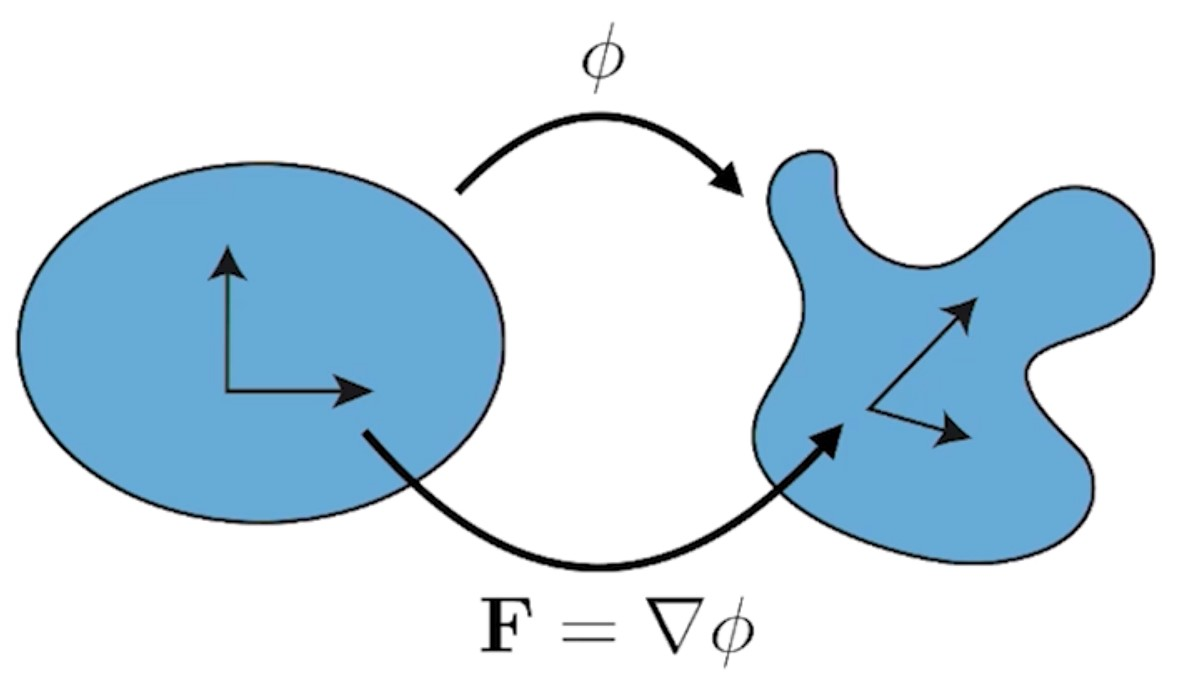
\includegraphics[width=0.5\textwidth]{resources/deformation_map}
	\caption[Deformation Map]{Deformation Map {\cite{STREAM2018}}}
	\label{fig:deformationmap}
\end{figure}

We can imagine that we map each particle of a chosen object from its rest state to a deformed one. Each particle $X$ of a body can be characterized by a vector $\mathbf{x}$ containing its positional coordinates at time $t_0=0$. This is the reference configuration. If the particles are displaced after a time $t$, we can describe their new coordinate vector with 
\[
	\check{\mathbf{x}} = \phi (\mathbf{x}, t).
\]
If we consider, for example a \textit{Translation}, every particle is displaced by the same distance and direction. Hence, we can calculate $\check{\mathbf{x}}$ with
\[
	\check{\mathbf{x}} = \mathbf{x} + \mathbf{c}(t)
\]
where $\mathbf{c}$ is a vector that only depends on $t$ (\cite{Spencer1980}, p.63).

\todoredefined[inline]{
TODO: Include own image instead of the one here? Other example than translation? Explain strain and stress more?
}


\subsection{Deformation Gradient}
The next quantity I will use in the upcoming chapters is the deformation gradient \textbf{F}. With its help, we can calculate the change in volume and length of an object during a deformation. We can obtain \textbf{F} by taking the gradient of the function $\phi$ discussed in the previous section.

\begin{wrapfigure}[11]{r}{5.5cm}
\centering
	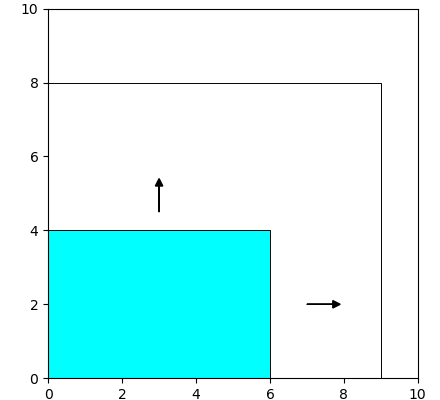
\includegraphics[width=5.5cm]{resources/stretch_plot.png}
	\caption[Stretching of a rectangle]{Stretching of a rectangle}
	\label{stretch:1}
\end{wrapfigure}
As an example, I am taking a simple deformation in 2D. The coloured area in Fig. \ref{stretch:1} represents an object in its rest state. We can stretch this area in the following way:
\begin{align*}
	\check{x} &= 1.5x + 0y		\\
	\check{y} &= 0x + 2y	
\end{align*}

The resulting deformation gradient can then be obtained by
\[
	\mathbf{F} = \begin{bmatrix} \frac{\partial [1.5x + 0y]}{\partial x} & \frac{\partial [1.5x + 0y]}{\partial y} \\ \frac{\partial [0x + 2y]}{\partial x} & \frac{\partial [0x + 2y]}{\partial y} \end{bmatrix} = \begin{bmatrix} 1.5 & 0.0 \\ 0.0 & 2.0 \end{bmatrix}.
\]
If \textbf{F} is equal to the identity matrix \textbf{I}, there is no deformation present. This would be the case for rigid body displacements. Since we will be handling deformation in the 3D space, the deformation gradient will have the form of a $3 \times 3$ matrix:
\begin{equation}\label{eq:deformation_gradient}
\textbf{F} = \left[ \,f_0\, \bigg| \,f_1\, \bigg| \,f_2\, \right] = \begin{bmatrix} f_0 & f_3 & f_6 \\ f_1 & f_4 & f_7 \\ f_2 & f_5 & f_8 \end{bmatrix}
\end{equation}
\textbf{F} can be factorized and used to calculate other quantities. The next few sections will explain this.

\subsubsection{Singular Value Decomposition of F}

Using the \acrshort{svd} theorem shown in Thm.\ref{SVD}, \textbf{F} can be written in the form of

\begin{equation}\label{eq:svd_gradient}
\mathbf{F} = \mathbf{U \Sigma V^\intercal}
\end{equation}

in which $\mathbf{\Sigma}$ stands for
\begin{equation}\label{eq:svd_simga}
\mathbf{\Sigma} = \left[\begin{matrix}  \sigma_0 & 0 & 0 \\ 0 & \sigma_1 & 0 \\ 0 & 0 & \sigma_2 \end{matrix}\right] .
\end{equation}

The $\sigma_i$ denote the singular values of $\mathbf{\Sigma}$.
\textbf{U} and $\mathbf{V}$ are both orthogonal matrices that represent the rotation of \textbf{F}. $\mathbf{\Sigma}$ on the other hand indicates the scaling of each coordinate $x_i$ by the factor $\sigma_i$. Unlike the standard convention, where a possible reflection lies in the rotation variants (meaning \textbf{U} and \textbf{V}), here the reflections are moved to $\mathbf{\Sigma}$ and it is therefore allowed to have a negative entry. This has the effect that $\operatorname{det}(\mathbf{U}) = \operatorname{det}(\mathbf{V}) =1$.


\subsubsection{Polar Decomposition of the Deformation Gradient}
With the help of Thm. \ref{PD} we can decompose the deformation gradient into the form
\begin{equation}\label{PD_DG}
	\mathbf{F} = \mathbf{RS},
\end{equation}
where \textbf{R} is orthogonal and \textbf{S} is a positive definite symmetric matrix. \textbf{R} symbolises the rotation (with possible reflection) that \textbf{F} undergoes, whereas \textbf{S} contains the scaling along the orthogonal directions of \textbf{F}.

\subsubsection{Relative volume change}
A useful information about a deformation is the relative volume change of the deformed object. It can be calculated by the determinate of \textbf{F}
\begin{equation}\label{det_DG}
	J = \operatorname{det}(\mathbf{F}).
\end{equation}
For a normal deformation, $J$ is a positive value. A determinant of zero would mean that the object is being deformed into a zero volume state, e.g. a plane or a point. A negative determinant indicates an inversion.


\subsubsection{Cauchy-Green}
The right Cauchy-Green tensor \textbf{C} can be calculated by 
\begin{equation}\label{CG_DG}
	\mathbf{C} = \mathbf{F^\intercal F},
\end{equation}
and is a $3 \times 3$ matrix for deformations in the 3D domain. Using \textbf{C}, we can calculate the first right Cauchy-Green invariant $I_C$ with
\begin{equation} \label{tr_CG_DG}
	I_C = \operatorname{tr}(\mathbf{C}).
\end{equation}
This quantity describes the length change of the object after a deformation.

\subsection{Deformation Energy}
The deformation energy or strain energy $\Psi$ is a scalar that defines the stored energy of a object undergoing a deformation. The strain energy density is the strain energy per unit volume. It equal to the work that has to be done by the stresses in order to alter the strains (\cite{KORSUNSKY20175}, p.10). This means that the energy is an indicator of how much force must be applied in order for an object to be deformed in a certain way. Thus, we can use the deformation energy to express the relationship between the stresses and strains. We can illustrate this with a stress-strain curve shown in Fig. \ref{fig:stress_strain}. The area under the stress-strain curve corresponds to the strain energy. 
\begin{figure}[!htbp]
	\centering
	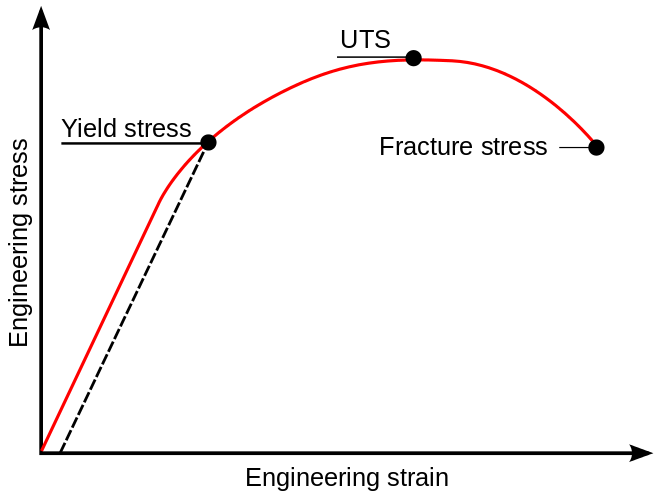
\includegraphics[width=0.5\textwidth]{resources/stress_strain_curve.png}
	\caption[Stress-strain curve]{Example for a stress-strain curve\footnotemark}
	\label{fig:stress_strain}
\end{figure}
\footnotetext{https://commons.wikimedia.org/wiki/File:Stress-strain\_curve.svg}

This relationship is not always linear. For example if we reach a stress state that produces yielding, we cannot assume that the relationship is linear anymore. If the material reaches the yield point, it can no longer recover into its rest shape due to permanent fractures during the deformation. This point is illustrated in Fig. \ref{fig:stress_strain} with \textit{Yield stress}. \textit{UTS} in Fig. \ref{fig:stress_strain} is abbreviated for Ultimate tensile strength and defines the maximal stress an object can bear before breaking. 


The behaviour of the object depends heavily on the material it consists of. This will be further explained in the next section concerning \textit{Material Constants}. In order to get a convincing simulation for a specific material, we have to choose an appropriate energy function. The behaviour of human flesh can be put into the category of hyperelastic materials. So we need a hyperelastic energy. The key property of elasticity is, that if all the forces that are applied over an object are removed, the object recovers into its original shape and volume (\cite{KORSUNSKY20175}, p. 5). For deformations of elastic materials, the Hooke's equation holds to some extend. Hooke's law describes a linear relationship of the applied force and the distance to the original position of a spring:
\[
	F = kx
\]
\textit{F} decribes the force, \textit{x} the distance and \textit{k} is a constant value. Material for which this equation holds are called linear-elastic or Hookean.

\todoredefined[inline]{
TODO: Explain Hooke better and add source for hookean, Neo-Hookean Model in Hyperelasticity. Not happy with last paragraph, maybe additional subsection?
}

\subsection{Material Constants}
When we look at a deformation of an object, we need to consider the material the object consists of. A material can be very stiff like steel or easily deformable like rubber. In order to measure the deformation of a specific material, we need the \textit{Poisson's Ratio} of said material. The poisson's ratio is a material constant that is defined as 

\begin{equation}\label{eq:poisson}
\sigma = - \frac{\epsilon_{11}}{\epsilon_{22}} \in [-1, 0.5]
\end{equation}

where $\epsilon_{11}$ is the lateral and $\epsilon_{22}$ the axial strain. The range in which $\sigma$ lies in starts at $-1$ and goes up to $0.5$ \cite{PhysRevB.80.132104}. If we imagine pulling a rubber band on each of its sides, we can observe that the band gets longer and the middle part gets narrower. The poisson's ratio indicates the extend of this process. Incompressible materials such as rubber lead to a higher poisson's ratio.

Usually the poisson's ratio of a material is positive. A negative value would mean that the material becomes wider in the cross section when it is stretched. This behaviour is very uncommon in nature. Examples of materials with a negative poisson's ratio are for instance discussed in \textit{Foam structures with a negative Poisson's ratio} \cite{lakes1987foam} or \textit{Advances in negative Poisson's ratio materials} \cite{lakes1993advances}. In table \ref{table:1} are some examples of the poisson's ratio of various materials.

\begin{table}[!htbp]
\centering
    \begin{tabular}{ | l | l |}
    \hline
    \textbf{Material} & \textbf{Poisson's ratio} \\ \hline
    C (graphite) & 0.31 \\ \hline
    Sn (metal) & 0.357 \\ \hline
    Cu & 0.355 \\ \hline
    Zn & 0.25 \\ \hline
    Ag & 0.36 \\ \hline
    Au & 0.45 \\ \hline
    Concrete & 0.20–0.37 \\ \hline
    Titanium (dental alloy) & 0.30–0.31 \\ \hline
    Bronze & 0.34 \\ \hline
    18–8 Stainless steel & 0.305 \\ \hline
    Natural rubber & 0.4999 \\ \hline
	B\textsubscript{2}O\textsubscript{3} glass & 0.30 \\ \hline
	GeO\textsubscript{2} glass & 0.20 \\ \hline	
    \end{tabular}
    \caption[Materials with their poisson's ratio]{Different materials with their poisson's ratio (\cite{PhysRevB.80.132104}, p. 3)}
\label{table:1}
\end{table}

In the context of flesh simulations, I am using the poisson's ratio as a characterization for the resistance to volume change of flesh. The poisson's ratio of biological tissues such as flesh, fat and muscles takes on higher values in the range of 0.45 and 0.5 (\cite{Smith:2018:SNF:3191713.3180491}, 12:1).

The calculation of the poisson's ratio defined in Eq. \ref{eq:poisson} is a challenge. Fortunately, we can make use of the \textit{Lamé Parameters}, the two material specific constants $\mu$ and $\lambda$. With the help of these two constants we can transform Eq. \ref{eq:poisson} into the form

\begin{equation}\label{eq:poisson_ratio}
\sigma =  \frac{\lambda}{2(\lambda + \mu)}.
\end{equation}

This equation allows to calculate the poisson's ratio much easier (\cite{BERGSTROM2015209}, p. 231). 


\todoredefined[inline]{
TODO: Include Piola-Kirchhoff Stress?
}





